\documentclass[conference]{IEEEtran}
\IEEEoverridecommandlockouts
% The preceding line is only needed to identify funding in the first footnote. If that is unneeded, please comment it out.
\usepackage{cite}
\usepackage{amsmath,amssymb,amsfonts}
\usepackage{algorithmic}
\usepackage{graphicx}
\usepackage{textcomp}
\usepackage{xcolor}
\usepackage{graphicx} % For including images
\usepackage{subcaption} % For subfigures
\usepackage{booktabs}
\usepackage{placeins} % For FloatBarrier
\def\BibTeX{{\rm B\kern-.05em{\sc i\kern-.025em b}\kern-.08em
    T\kern-.1667em\lower.7ex\hbox{E}\kern-.125emX}}
\begin{document}

\title{Cardiovascular Disease Prediction}


\author{\IEEEauthorblockN{1\textsuperscript{st} Peifan Bai}
\IEEEauthorblockA{\textit{Department of Computer Science} \\
\textit{University of Western Ontario}\\
London, ON \\
pbai8@uwo.ca}

}

\maketitle

\begin{abstract}

\end{abstract}

\begin{IEEEkeywords}

\end{IEEEkeywords}

\section{Introduction}


\section{Methodology}

XGBoost (eXtreme Gradient Boosting) models were employed for both cardiovascular disease classification and systolic blood pressure regression tasks~\cite{chen2016xgboost}. The classification model utilizes logistic loss with sigmoid activation for binary prediction, while the regression model employs squared loss for continuous output. Both models incorporate identical tree structure optimization algorithms with regularization terms to prevent overfitting, which are detailed in Appendix~\ref{sec:xgboost_formulas}.

\section{Data Processing}

The cardiovascular disease dataset underwent rigorous purification, reducing 70,000 initial records to 68,425 valid samples after eliminating physiologically implausible values~\cite{cardiovascular_dataset}, as shown in Figure~\ref{fig:data_cleaning_process} of Appendix~\ref{sec:data_cleaning}. Engineered features included BMI calculations, blood pressure categorizations, and composite risk scores. Numerical features were z-score normalized, while categorical features underwent one-hot encoding, yielding 19 final features (6 numerical, 13 categorical). The dataset was stratified into training (80\%), validation (10\%), and test (10\%) sets. Detailed feature engineering specifications appear in Table~\ref{tab:feature_engineering} of Appendix~\ref{sec:feature_engineering}.

\section{Results}

\subsection{Model Performance}
Hyperparameter optimization via grid search with cross-validation yielded distinct configurations for each task (see Table~\ref{tab:hyperparameters} of Appendix~\ref{sec:xgboost_classification} for details). The classification model achieved 82.1\% ROC-AUC with 86.5\% recall, demonstrating exceptional discriminative capability for cardiovascular disease detection. The regression model attained R² = 58.9\% with RMSE = 10.80 mmHg for systolic pressure prediction, as shown in Tables~\ref{tab:classification_metrics} and~\ref{tab:regression_metrics}, which are visualized through Figures~\ref{fig:confusion_matrices}--\ref{fig:true_vs_predicted} in Appendix~\ref{sec:performance_metrics} showing model diagnostic performance across classification and regression tasks.
\begin{table}[h]
\centering
\caption{Classification Performance Metrics}
\label{tab:classification_metrics}
\begin{center}
\begin{tabular}{p{2.5cm}p{2cm}p{2cm}}
\toprule
\textbf{Metric} & \textbf{Training} & \textbf{Test} \\
\midrule
Accuracy & 70.4\% & 71.7\% \\
Precision & 65.4\% & 66.4\% \\
Recall & 85.1\% & 86.5\% \\
F1-Score & 74.0\% & 75.2\% \\
ROC-AUC & 80.7\% & 82.1\% \\
Average Precision & 79.5\% & 80.5\% \\
Specificity & 55.9\% & 57.2\% \\
\bottomrule
\end{tabular}
\end{center}
\end{table}

\begin{table}[h]
\centering
\caption{Regression Performance Metrics}
\label{tab:regression_metrics}
\begin{center}
\begin{tabular}{p{3cm}p{2cm}p{2cm}}
\toprule
\textbf{Metric} & \textbf{Training} & \textbf{Test} \\
\midrule
MAE (mmHg) & 7.28 & 7.39 \\
RMSE (mmHg) & 10.63 & 10.80 \\
R² Score & 59.3\% & 58.9\% \\
MSE & 113.07 & 116.56 \\
\bottomrule
\end{tabular}
\end{center}
\end{table}
\subsection{Feature Importance Analysis}
Feauture importance analysis revealed four distinct patterns of feature utilization that illuminate the complementary nature of classification and regression modeling approaches, as quantified in Table~\ref{tab:feature_importance_comparison}~\cite{lundberg2017unified}:

\subsubsection{Shared Core Risk Factors} 
Both models demonstrate convergent prioritization of systolic blood pressure (\texttt{ap\_hi}) and cholesterol as critical predictive elements. Systolic pressure achieves rank 2 in classification (importance: 0.256) and rank 1 in regression (importance: 0.745), demonstrating its fundamental role across both tasks with substantially greater influence on continuous BP prediction. Cholesterol maintains consistent relevance with rank 3 in classification (importance: 0.087) and rank 5 in regression (importance: 0.036), representing a truly shared physiological risk indicator with balanced influence across modeling approaches.

\subsubsection{Classifier-Specific Drivers} 
Categorical hypertension indicators demonstrate stark task-specific importance patterns. \texttt{BP\_Category\_Hypertension} dominates CVD classification with rank 1 (importance: 0.461) but becomes virtually irrelevant for regression (rank 19, importance: $<$1E-04), yielding a rank difference of 18. Similarly, \texttt{bp\_category} achieves rank 4 in classification (importance: 0.066) while ranking 19th in regression (rank difference: 15). This pattern confirms the classifier's reliance on discrete hypertension thresholds, which the regressor circumvents through direct continuous BP modeling.

\subsubsection{Regressor-Specific Insights} 
Interaction features exhibit pronounced specificity for BP prediction. Age-weight interaction achieves rank 2 in regression (importance: 0.053) but rank 14 in classification (importance: $<$1E-04), demonstrating a rank difference of -12. Age-BMI interaction (rank 3 regression vs. rank 14 classification, difference: -11) and cholesterol-glucose interaction (rank 4 regression vs. rank 14 classification, difference: -10) follow similar patterns. These composite terms substantially shape BP prediction while remaining peripheral to CVD classification, revealing physiological nuances wherein BP responds to combined effects of age, body composition, and metabolic interactions.

\subsubsection{Clinical Implications} 
The quantitative analysis validates dual modeling utility through complementary feature importance patterns. Features with rank differences exceeding 10 (BP categorical indicators and interaction terms) demonstrate task-specific specialization, while features with minimal rank differences (cholesterol: 2, age: 1) represent shared physiological mechanisms. This complementary information capture enables enhanced risk stratification when models are employed synergistically.

Comprehensive feature importance visualizations and quantitative comparisons appear in Appendix~\ref{sec:feature_analysis} (Tables~\ref{tab:feature_importance_comparison}, Figures~\ref{fig:model_importance_scatter}-\ref{fig:model_importance_dumbbell}). The concordance between model-identified features and established clinical guidelines validates the interpretability and clinical relevance of the proposed methodology~\cite{whelton2017acc,goff2014acc}.

\FloatBarrier



\newpage
\bibliographystyle{IEEEtran}
\bibliography{references}
\appendix

\subsection{Mathematical Formulations}
\label{sec:xgboost_formulas}

\subsubsection{XGBoost Classification Model}
\label{sec:xgboost_classification}
The objective function for XGBoost Classification Model is given by:
\begin{equation}\label{eq:XGBoostClassObjective}
\mathcal{L} = \sum_{i=1}^{n} l(y_i, \hat{y}_i) + \sum_{k=1}^{K} \Omega(f_k),
\end{equation}
where $l(y_i, \hat{y}_i)=-[y_i \log(\hat{y}_i) + (1-y_i) \log(1-\hat{y}_i)]$ is the logistic loss function with $y_i$ being the true label and $\hat{y}_i$ the predicted probability, and $\Omega(f_k) = \gamma T + \frac{1}{2}\lambda \sum_{j=1}^{T} w_j^2$ is the regularization term.

The prediction for instance $i$ is given by:
\begin{equation}
\hat{y}_i = \sigma\left(\sum_{k=1}^{K} f_k(x_i)\right),
\end{equation}
where $\sigma(z) = \frac{1}{1 + e^{-z}}$ is the sigmoid function.

\subsubsection{XGBoost Regression Model}
The objective function for XGBoost Regression Model is given by:
\begin{equation}\label{eq:XGBoostRegObjective}
\mathcal{L} = \sum_{i=1}^{n} l(y_i, \hat{y}_i) + \sum_{k=1}^{K} \Omega(f_k),
\end{equation}
where $l(y_i, \hat{y}_i) = \frac{1}{2}(y_i - \hat{y}_i)^2$ is the squared loss function.

\subsection{Data Cleaning Process}
\label{sec:data_cleaning}

The comprehensive data cleaning pipeline transformed the raw cardiovascular dataset through systematic quality assurance and feature engineering steps, as illustrated in Figure~\ref{fig:data_cleaning_process}. The process began with 70,000 raw records and yielded 68,425 validated samples suitable for machine learning analysis.

\begin{figure}[h]
    \centering
    
    \begin{minipage}{0.48\textwidth}
        \centering
        \textbf{Data Cleaning Pipeline}
        \vspace{0.3cm}
        
        \fbox{\parbox{0.9\textwidth}{
            \centering
            \textbf{Raw Dataset} \\
            70,000 records \\
            12 features
        }}
        
        \vspace{0.2cm}
        $\downarrow$
        
        \fbox{\parbox{0.9\textwidth}{
            \centering
            \textbf{Step 1: Age Conversion} \\
            Days $\rightarrow$ Years \\
            age\_years = age / 365.25
        }}
        
        \vspace{0.2cm}
        $\downarrow$
        
        \fbox{\parbox{0.9\textwidth}{
            \centering
            \textbf{Step 2: Physical Outlier Removal} \\
            Height: 140-220 cm \\
            Weight: 40-200 kg
        }}
        
        \vspace{0.2cm}
        $\downarrow$
        
        \fbox{\parbox{0.9\textwidth}{
            \centering
            \textbf{Step 3: Blood Pressure Validation} \\
            Systolic: 80-220 mmHg \\
            Diastolic: 40-120 mmHg \\
            Constraint: \texttt{ap\_hi} $>$ \texttt{ap\_lo}
        }}
        
        \vspace{0.2cm}
        $\downarrow$
        
        \fbox{\parbox{0.9\textwidth}{
            \centering
            \textbf{Step 4: Feature Engineering} \\
            BMI Calculation \\
            BP Categories \\
            Risk Factor Scoring\\
            Interaction Features
        }}
        
        \vspace{0.2cm}
        $\downarrow$
        
        \fbox{\parbox{0.9\textwidth}{
            \centering
            \textbf{Step 5: Data Preprocessing} \\
            Standardization \\
            One-Hot Encoding \\
            Train/Validation/Test Split
        }}
        
        \vspace{0.2cm}
        $\downarrow$
        
        \fbox{\parbox{0.9\textwidth}{
            \centering
            \textbf{Clean Dataset} \\
            68,425 records \\
            19 engineered features
        }}
    \end{minipage}
    \caption{Data cleaning and preprocessing pipeline flowchart showing the systematic transformation from raw cardiovascular data to model-ready features.}
    \label{fig:data_cleaning_process}
\end{figure}

\subsection{Performance Tables and Figures}
\label{sec:performance_metrics}
The performance of the models is summarized in Table~\ref{tab:hyperparameters} for hyperparameter configurations, and visualized through Figures~\ref{fig:confusion_matrices}--\ref{fig:true_vs_predicted} showing model diagnostic performance across classification and regression tasks.
\begin{table}[h]
\centering
\caption{Optimal Hyperparameters for XGBoost Models}
\label{tab:hyperparameters}
\begin{center}
\begin{tabular}{p{3cm}p{2cm}p{2cm}}
\toprule
\textbf{Parameter} & \textbf{Classification} & \textbf{Regression} \\
\midrule
Learning Rate & 0.05 & 0.05 \\
Max Depth & 5 & 3 \\
N Estimators & 300 & 300 \\
Subsample & 0.8 & 0.9 \\
Colsample Bytree & 0.8 & 1.0 \\
Reg Alpha (L1) & 0.1 & 1.0 \\
Reg Lambda (L2) & 5.0 & 2.5 \\
Gamma & 5.0 & -- \\
Min Child Weight & -- & 1.0 \\
\bottomrule
\end{tabular}
\end{center}
\end{table}



\begin{figure}[h]
    \centering
    \includegraphics[width=0.45\textwidth]{plots/confusion_matrices.pdf}
    \caption{Confusion matrices for cardiovascular disease classification models.}
    \label{fig:confusion_matrices}
\end{figure}

\begin{figure}[h]
    \centering
    \includegraphics[width=0.45\textwidth]{plots/precision_recall_comparison.pdf}
    \caption{Precision-recall curves comparing classification model configurations.}
    \label{fig:precision_recall}
\end{figure}

\begin{figure}[h]
    \centering
    \includegraphics[width=0.45\textwidth]{plots/roc_comparison.pdf}
    \caption{ROC curves showing diagnostic ability of classification models.}
    \label{fig:roc_comparison}
\end{figure}

\begin{figure}[h]
    \centering
    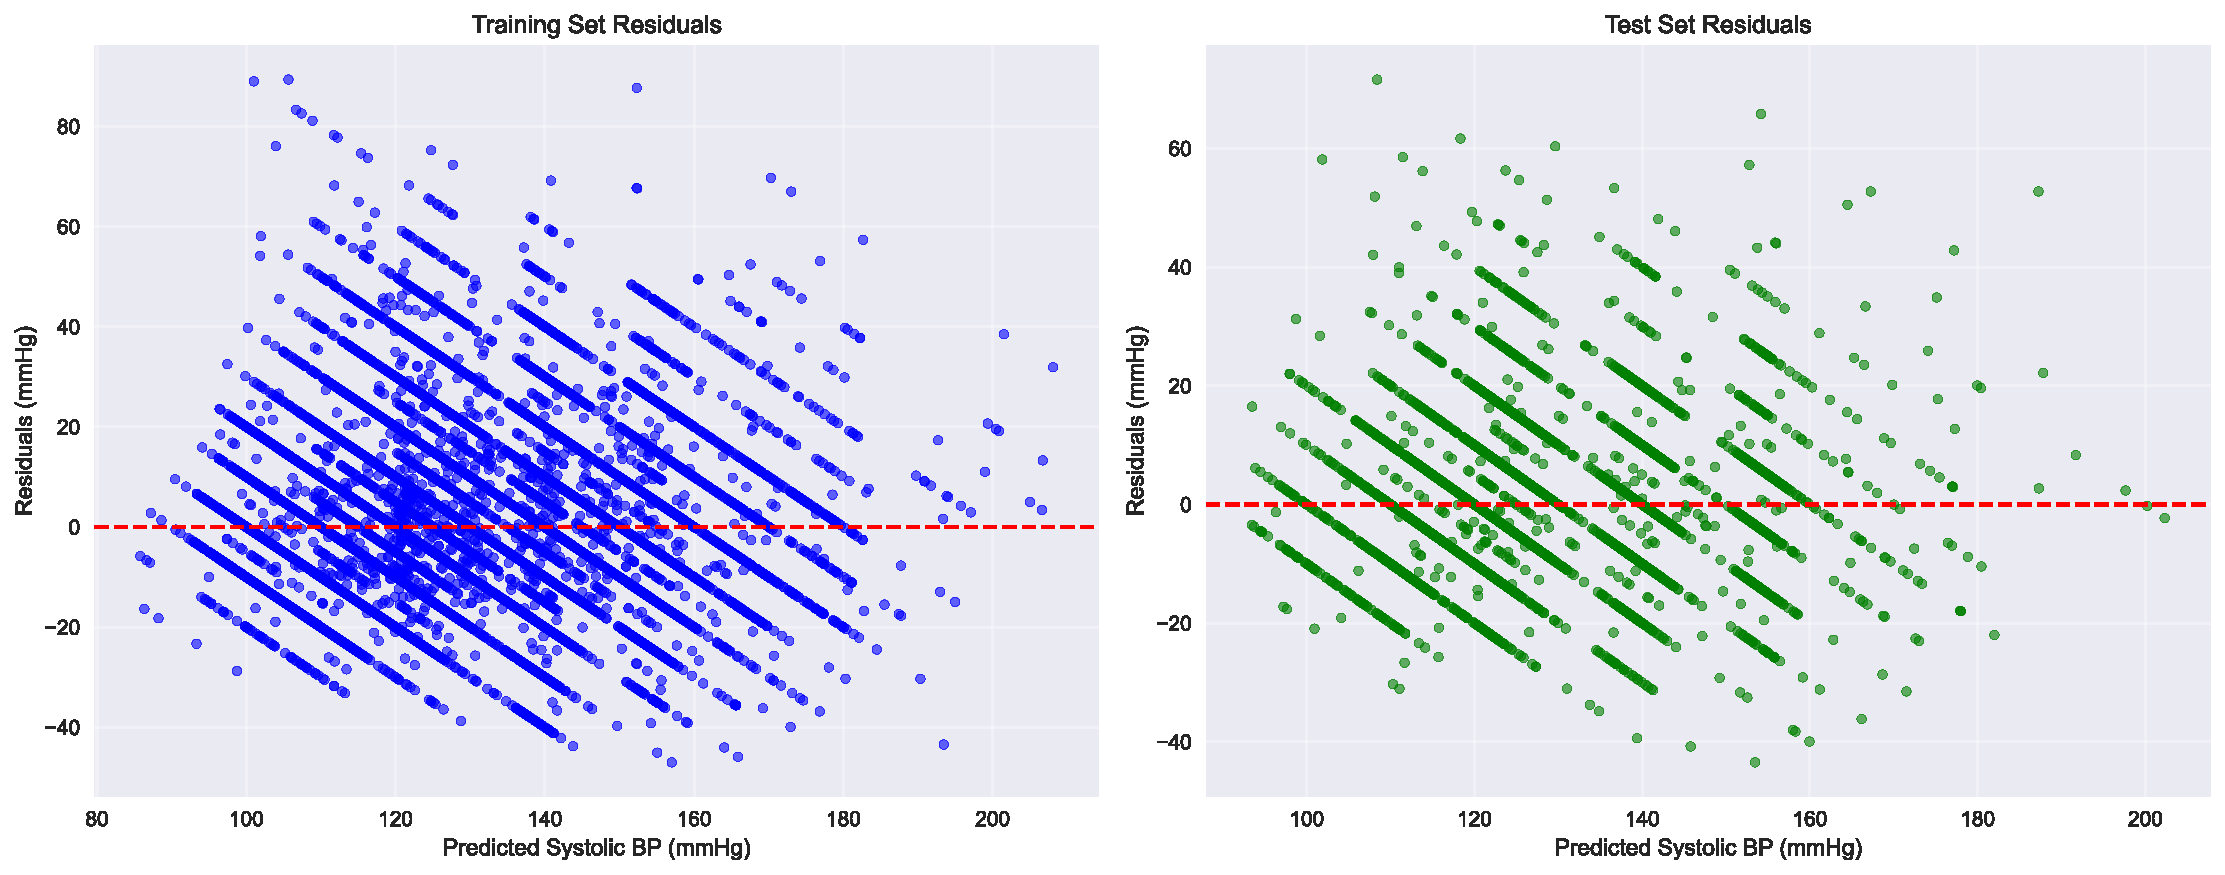
\includegraphics[width=0.45\textwidth]{plots/residual_plots.pdf}
    \caption{Residual plots for regression models showing error distributions.}
    \label{fig:residual_plots}
\end{figure}

\begin{figure}[h]
    \centering
    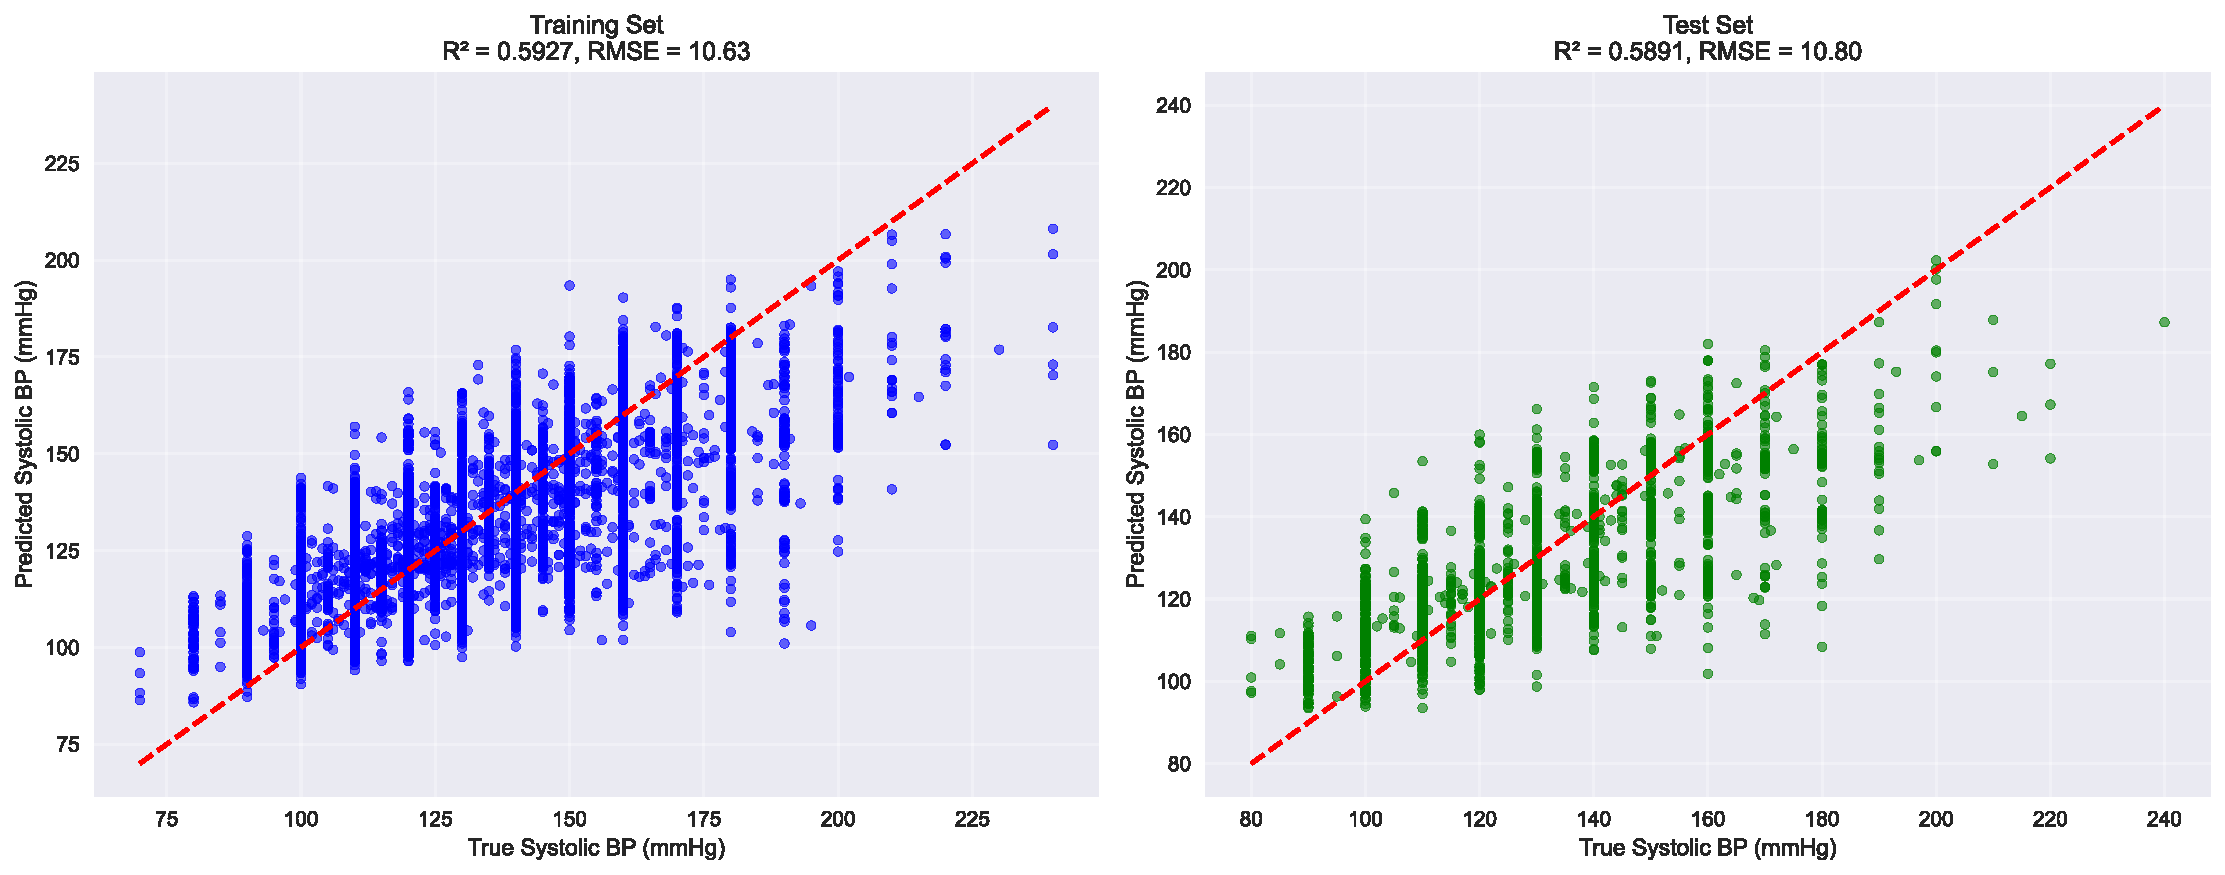
\includegraphics[width=0.45\textwidth]{plots/true_vs_predicted.pdf}
    \caption{True vs. predicted values correlation for regression model.}
    \label{fig:true_vs_predicted}
\end{figure}

\subsection{Feature Engineering and Analysis}
\label{sec:feature_analysis}
\label{sec:feature_engineering}
The feature engineering process involved several transformations and calculations to enhance model performance, as detailed in Table~\ref{tab:feature_engineering}. Cross-model feature importance analysis is presented in Table~\ref{tab:feature_importance_comparison}, with complementary visualizations in Figures~\ref{fig:model_importance_scatter} and~\ref{fig:model_importance_dumbbell} illustrating the comparative importance patterns between classification and regression models.
\begin{table*}[h]
\centering
\caption{Feature Engineering Transformations and Calculations}
\label{tab:feature_engineering}
\begin{center}
\begin{tabular}{p{3cm}p{6cm}p{8cm}}
\toprule
\textbf{Feature} & \textbf{Description} & \textbf{Calculation} \\
\midrule
BMI & Body Mass Index calculated from height and weight & $\text{BMI} = \frac{\text{weight}}{(\text{height}/100)^2}$ \\
\addlinespace
Age Groups & Age categorization for stratified analysis & $\text{Age Group} = \begin{cases}
\text{Young} & \text{if age} < 40 \\
\text{Middle} & \text{if } 40 \leq \text{age} < 60 \\
\text{Senior} & \text{if age} \geq 60
\end{cases}$ \\
\addlinespace
BP Category & Blood pressure categorization based on clinical guidelines & $\text{BP}_{\text{category}} = \begin{cases}
\text{Normal} & \text{if SBP} < 120 \text{ and DBP} < 80 \\
\text{Elevated} & \text{if } 120 \leq \text{SBP} < 130 \text{ and DBP} < 80 \\
\text{Stage 1 HTN} & \text{if } 130 \leq \text{SBP} < 140 \text{ or } 80 \leq \text{DBP} < 90 \\
\text{Stage 2 HTN} & \text{if SBP} \geq 140 \text{ or DBP} \geq 90
\end{cases}$ \\
\addlinespace
Age-Weight Interaction & Age-weight interaction term for cardiovascular risk modeling & $\text{age\_weight\_interaction} = \text{age} \times \text{weight}$ \\
Age-BMI Interaction & Age-BMI interaction term & $\text{age} \times \text{BMI}$ \\
Cholesterol-Glucose & Cholesterol-glucose interaction for metabolic risk assessment & $\text{cholesterol} \times \text{glucose}$ \\
\addlinespace
Pulse Pressure & Difference between systolic and diastolic blood pressure & $\text{pulse\_pressure} = \text{ap\_hi} - \text{ap\_lo}$ \\
Mean Blood Pressure & Estimated mean arterial pressure using clinical formula & $\text{mean\_bp} = \frac{\text{ap\_hi} + 2 \times \text{ap\_lo}}{3}$ \\
\bottomrule
\end{tabular}
\end{center}
\end{table*}

\begin{table*}[h]
\centering
\caption{Cross-Model Feature Importance Comparison}
\label{tab:feature_importance_comparison}
\begin{center}
\begin{tabular}{p{3.5cm}p{2cm}p{2cm}p{1.5cm}p{1.5cm}p{1.5cm}}
\toprule
& \multicolumn{2}{c}{\textbf{Importance}} &  \multicolumn{3}{c}{\textbf{Rank}} \\
\cmidrule(lr){2-3} \cmidrule(lr){4-6}
\textbf{Feature} & \textbf{Classification} &  \textbf{Regression}& \textbf{Classification} &  \textbf{Regression} & \textbf{Difference} \\
\midrule
BP Category Hypertension & 0.461 & $<$1E-04 & 1 & 19 & 18 \\
Systolic Pressure (ap\_hi) & 0.256 & 0.745 & 2 & 1 & -1 \\
Cholesterol & 0.087 & 0.036 & 3 & 5 & 2 \\
BP Category & 0.066 & $<$1E-04 & 4 & 19 & 15 \\
Age & 0.047 & 0.012 & 5 & 6 & 1 \\
Glucose & 0.017 & 0.010 & 6 & 8 & 2 \\
Physical Activity & 0.016 & 0.005 & 7 & 13 & 6 \\
Weight & 0.012 & 0.006 & 8 & 10 & 2 \\
Smoking & 0.010 & 0.002 & 9 & 18 & 9 \\
Alcohol & 0.010 & $<$1E-04 & 10 & 19 & 9 \\
BMI & 0.007 & 0.005 & 11 & 14 & 3 \\
Gender & 0.006 & 0.012 & 12 & 7 & -5 \\
Height & 0.004 & 0.006 & 13 & 11 & -2 \\
Age-Weight Interaction & $<$1E-04 & 0.053 & 14 & 2 & -12 \\
Age-BMI Interaction & $<$1E-04 & 0.045 & 14 & 3 & -11 \\
Cholesterol-Glucose & $<$1E-04 & 0.040 & 14 & 4 & -10 \\
\bottomrule
\end{tabular}
\end{center}
\end{table*}

\begin{figure}[h]
    \centering
    \includegraphics[width=0.45\textwidth]{plots/model_importance_scatter.pdf}
    \caption{Scatter plot comparing normalized feature importance between cardiovascular disease classifier and systolic blood pressure regressor.}
    \label{fig:model_importance_scatter}
\end{figure}

\begin{figure}[h]
    \centering
    \includegraphics[width=0.45\textwidth]{plots/model_importance_dumbbell.pdf}
    \caption{Dumbbell chart comparing feature importance between models for the top 15 features.}
    \label{fig:model_importance_dumbbell}
\end{figure}

\subsection{Author's contribution}

Peifan Bai executed the implementation and optimization of XGBoost classification and regression models, encompassing feature importance analysis using feature importance values for model interpretability, comprehensive comparison analysis, and visualizations for Figures~\ref{fig:data_cleaning_process}, \ref{fig:confusion_matrices}, \ref{fig:precision_recall}, \ref{fig:roc_comparison}, \ref{fig:residual_plots}, \ref{fig:true_vs_predicted}, \ref{fig:model_importance_scatter}, and \ref{fig:model_importance_dumbbell}, as well as Tables~\ref{tab:classification_metrics}, \ref{tab:regression_metrics}, \ref{tab:hyperparameters}, \ref{tab:feature_engineering}, and \ref{tab:feature_importance_comparison}.

\subsection{Acknowledgments}

The authors acknowledge that Artificial Intelligence (AI) tools were used solely for debugging code issues and grammar checking during the preparation of this manuscript.



\end{document}
